\section{Auswertung}

Als erstes haben wir den Laser, den Drehmotor und den Oszillator eingeschaltet. Dann haben wir die korrekte Justierung aller Spiegel überprüft und den 4.Spiegel richtig eingestellt. Nach Einschalten des Computers und des Periodenzählers haben wir dann noch die Blendenöffnung optimiert, sodass auf dem Oszilloskopen ein klares, etwa sinusförmiges Signal erkennbar war. Bei den jeweiligen Messungen haben wir die Skala des Oszillators immer wieder angepasst und mit Hilfe der \emph{HOLD}-Taste haben wir uns immer ein Bild herausgesucht, welches optimal für die Auswertung geeignet war. Gleichzeitig haben wir die Rotationsperiode der Quarzscheibe am Periodenzähler abgelesen und aufgeschrieben.

Im ersten Versuchsteil stellen wir eine feste Periode der Quarzscheibe anhand der Spannung am Drehmotor ein und variieren den Durchtrittspunkt durch die Scheibe. Dies machen wir für 4 feste Perioden. Im zweiten Versuchsteil, legen wir 4 verschiedene Durchtrittspunkte fest, für die wir jeweils die Periode verändern und dann messen.

\subsection{Berechnung des Fehlers auf die Periode der Scheibe}

In dem ersten Teil mit der festen Drehzahl haben wir bei jeder Messung diese jeweils immer auch gemessen um den Fehler berechnen zu können. Die Werte kann man im Anhang einsehen. Für die Mittelwerte der Drehzahlen und deren Standardabweichung haben wir folgende Werte berechnet:

\begin{center}
\begin{tabular}[H]{c c}
$P_{5V}=(90401 \pm 963) \mu s$ & $P_{7,5V}=(50776 \pm 591) \mu s$ \\
 & \\
$P_{8,5V}=(45385 \pm 919) \mu s$ & $P_{10V}=(34865 \pm 311) \mu s$
\end{tabular}
\end{center}

Wir werden weiterhin die Spannung als Referenz für diese Größen benutzen, da dies einfach übersichtlicher ist.

Aus diesen Perioden folgen die Winkelfrequenzen der Quarzscheibe durch die Formel

$$\omega = \frac{2\pi}{P}   \text{ \ \ mit dem Fehler \ \ } 
\sigma_\omega = \left|\frac{\partial \omega}{\partial P}\sigma_P\right| = \frac{2\pi\sigma_P}{P^2}$$

Somit ergeben sich:

\begin{center}
\begin{tabular}[H]{c c}
$\omega_{5V} = (69,50 \pm 0,74) Hz$ & $\omega_{7,5V} = (123,74 \pm 1,44) Hz$\\
 & \\
$\omega_{8,5V} = (138,44 \pm 2,80) Hz$ & $\omega_{10V} = (180,22 \pm 1,61) Hz$
\end{tabular}
\end{center}

Hieraus können wir den Fehler auf die Periode (und somit auch die Frequenz) abschätzen. Wir schätzen ihn allgemein auf 1,2\% des Wertes.

\clearpage
%--------

\subsection{Bestimmung des Nullpunktes der Quarzscheibe}

Indem wir die Schwebungsfrequenz gegen den Durchtrittspunkt in einem Graphen auftragen, können wir durch lineare Regression berechnen, an welcher Stelle das Licht durch das Zentrum der Quarzscheibe durchtritt. Der Achsenabschnitt ist nämlich genau dieser Nullpunkt.

Wir erhalten für die Achsenabschnitte und somit für die Nullpunkte 

\begin{center}
\begin{tabular}[H]{c c}
$x_0^{5V} = (46,90 \pm 0,15) mm$ & $x_0^{7,5V} = (46,32 \pm 0,05) mm$\\
 & \\
$x_0^{8,5V} = (46,26 \pm 0,05) mm$ & $x_0^{10V}= (46,45 \pm 0,04) mm$
\end{tabular}
\end{center}


und berechnen daraus den gewichteten Mittelwert und den Fehler darauf mit den Formeln:

$$\bar x = \frac{\sum_{i=1}^{N} \frac{x_i}{\sigma_i^2}}{\sum_{i=1}^{N} \frac{1}{\sigma_i^2}} \text{ \ \ und \ \ } 
\sigma_{\bar x} = \left(\sum_{i=1}^{N} \frac{1}{\sigma_i^2}\right)^{-1} $$

mit $\sigma_i = \sigma_{x_0} = 10^{-3} mm$. Es folgt also: 

$$\boxed{\bar x = (46,377 \pm 0,001) mm}$$

\begin{figure}[H]
	\centering 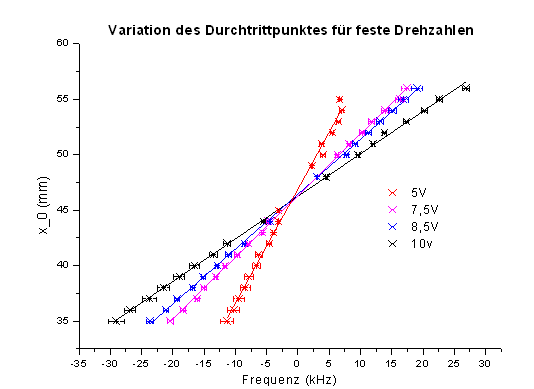
\includegraphics[width = 0.99\textwidth]{Bilder/graph1.jpg}
	\caption{Variation von $x_0$}
\end{figure}

Wichtig ist hier zu bemerken, dass wir die Werte um den Nullpunkt zu einem großen Teil vernachlässigt haben, da das Bild am Oszilloskop so ungenau war, dass wir kaum noch sinusförmige Strukturen erkennen konnten und die Periode somit wahrscheinlich eher geraten haben. Wir haben somit die meisten dieser Werte einfach verworfen.

\subsection{Berechnung von $\alpha$ durch Variation des Durchtrittspunktes}

Der Mitführungskoeffizient $\alpha$ lässt sich durch folgende Formel berechnen:

$$\alpha = \frac{L\cdot\lambda\cdot\Delta\nu}{2\cdot n\cdot\omega\cdot d \cdot x_0}$$

Wichtig ist, dass hier das $x_0$ in der Formel in unserem Fall eigentlich $x_0 - \bar x$ ist, da der Nullpunkt ja nicht bei Null, sondern bei $\bar x$ liegt.\\

Wir kennen die Werte\\

\begin{tabular}[H]{l}
$L = 2,149 m$, optische Gesamtlänge des Resonators\\
$\lambda = 6,3282\cdot10^{-7} m$ Wellenlänge des Laserlichts\\
$n = 1,457$ Brechungsindex des Quarzes\\
$d = 0,0127 m$ Dicke der Quarzscheibe
\end{tabular}\\


da sie angegeben sind. Wir nehmen den Fehler auf diese Größen als vernachlässigbar klein an. Wir berechnen $\alpha$ für jede einzelne Messgröße und berechnen den statistischen Fehler, da der Fehler durch die Fortpflanzung so klein ist, dass seine Aussage keinen Sinn mehr macht (Bereich $\sim 10^{-4}$  bis  $10^{-5}$). Der statistische Fehler ist aber auch sehr klein, was wahrscheinlich daran liegt, dass wir die stark abweichenden Werte in der Nähe des Nullpunktes der Scheibe komplett vernachlässigt haben. Wir erhalten die Werte

\begin{center}
\begin{tabular}[H]{c c}
	$\alpha_{5V} = 0,536 \pm 0,073$ & $\alpha_{7,5V} = 0,535 \pm 0,023$\\
	 & \\
	$\alpha_{8,5V} = 0,532 \pm 0,018$ & $\alpha_{10V} = 0,528 \pm 0,024$
\end{tabular}
\end{center}

und somit hieraus den gewichteten Mittelwert mit Fehler:

$$\boxed{\alpha_1 =0,5319 \pm 0,0001}$$

\clearpage
%----------

\subsection{Berechnung von $\alpha$ durch Variation der Drehfrequenz}

Aus der Formel (11) für $\alpha$, folgt, dass $$\Delta\nu = \frac{x_0\cdot\alpha}{c}\cdot\omega \text{\ \ wobei \ \ }
c = \frac{L\lambda}{2nd} = 3,67\cdot 10^{-5}$$

Wir haben also $\Delta\nu$ gegen $f=\omega/2\pi$ aufgetragen und aus der Steigung $b=\frac{x_0\alpha}{c}$ haben wir $\alpha$ berechnet, also $\alpha=\frac{c\cdot b}{x_0}$. Jedoch müssen wir noch einen Faktor $2\pi$ in die Formel für $\alpha$ integrieren, da wir den Graphen gegen $f$ und nicht gegen $\omega$ aufgetragen haben, somit folgt $$\alpha = \frac{c\cdot b}{2\pi x_0}$$

\begin{figure}[H]
	\centering 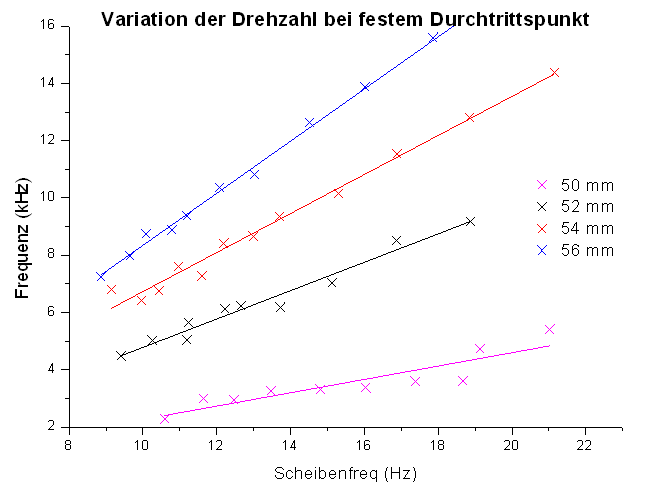
\includegraphics[width = \textwidth]{Bilder/graph2.jpg}
	\caption{Variation von $\omega$}
\end{figure}




Für die 4 Steigungen erhalten wir:

\begin{center}
\begin{tabular}[H]{c c}
	$b_{50mm} = 233,0 \pm 39,0 $ & $b_{52mm} = 495,5 \pm 31,5$\\
	 & \\
	$b_{54mm} = 681,4 \pm 25,7 $ & $b_{56mm} = 909,8 \pm 14,6$
\end{tabular}
\end{center}

Die Achsenabschnitte liegen alle innerhalb des Fehlers um Null. Nur der Achsenabschnitt für $x_0 = 56mm$ liegt in der 4. Standardabweichung des Fehlers.

Der Fehler auf $\alpha$ ergibt sich durch:
$$\sigma_\alpha = \alpha\cdot\sqrt{\frac{\sigma^2_{x_0}}{x_0^2}+\frac{\sigma_b^2}{b^2}} = \alpha\cdot\frac{\sigma{b}}{b}$$
Der relative Fehler von $x_0$ ist viel kleiner als der von $b$ und somit vernachlässigbar.

Für die 4 verschiedenen Durchtrittspunkte erhalten wir die Mitführungskoeffizienten:


\begin{center}
\begin{tabular}[H]{c c}
	$\alpha_{50mm} = 0,3756 \pm 0,0629 $ & $\alpha_{52mm} = 0,51471 \pm 0,0327$\\
	 & \\
	$\alpha_{54mm} = 0,52211 \pm 0,0197 $ & $\alpha_{56mm} = 0,55223 \pm 0,0089$
\end{tabular}
\end{center}

Als gewichteten Mittelwert dieser Werte erhalten wir:

$$\boxed{\alpha_2 = 0,5427 \pm  0,0001}$$

\subsection{Theoretische Berechnung von $\alpha$ und Vergleich}

Der theoretische Wert von $\alpha$ lautet:

$$\alpha = 1 - \frac{1}{n^2} - \frac{\lambda\cdot\Delta n}{n \cdot\Delta\lambda} = 0,541965$$

mit $$\frac{\Delta n}{\Delta\lambda} = -300cm^{-1} = -30000m^{-1} \text{ \ gegeben}$$\\

Als Vergleich:

$\alpha_1 = 0,5319$ weicht um 1,9\% von diesem Wert ab, und $\alpha_2=0,5427$ nur um 0,1\%. Aussagen über die Standardabweichung sind irrelevant, da diese sehr klein sind und somit der theoretische Wert innerhalb von 101 bzw. 10 von den gemessenen Werten liegt.

\clearpage
%--------









